\documentclass{article}
\usepackage[a4paper, top=2cm, bottom=2cm, left=2.5cm, right=2.5cm]{geometry}
\usepackage{graphicx}
\usepackage{float}
\usepackage[dvipsnames]{xcolor}
\title{Intelligenza Artificiale I}
\author{Federico Falcone}
\date{\today}
\begin{document}
\maketitle
\section{Agenti}
\subsection{Agenti e ambienti}
Un \textbf{agente} è qualsiasi cosa possa essere vista come un sistema che percepisce il suo \textbf{ambiente} attraverso i \textbf{sensori} e agisce su di esso mediante \textbf{attuatori}.
Usiamo il termine \textbf{percezione} per indicare i dati che i sensori di un agente percepiscono. La \textbf{sequenzza percettiva} di un agente è la storia completa di tutto ciò che esso ha percepito nella sua esistenza. In generale, \textit{la scelta dell'azione di un agente in un qualsiasi istante può dipendere dalla conoscenscena integrata in esso e dall'intera sequenza percettiva osservata fino a quel punto, ma non da qualcosa che l'agente non abbia percepito}. Il comportamento di un agente quindi è descritto dalla \textbf{funzione agente}, che descrive la corrispondenza tra una qualsiasi sequenza percettiva e una specifica azione. \\
Possiamo immaginare di rappresentare in forma di \textbf{tabella}  la funzione agente che descrive un certo agente. La tabella è una descrizione \textbf{esterna} dell'agente. \textbf{Internamente}, la funzione agente di un agente artificiale sarà implementata da un \textbf{programma agente}, il quale è l'implementazione della funzione agente.

\subsection{Comportarsi correttamente: il concetto di razionalità}
Un \textbf{aagente razionale} è un agente che fa la cosa giusta.
\subsubsection{Misure di prestazione}
Valutiamo il comportamento di un agente considerandone le \textit{conseguenze}. Ciò si chiama \textbf{consequenzialismo}. Quando un agente viene inserito in un ambiente, genera una sequenza di azioni in base alle percezioni che riceve. Questa sequenza di azioni porta l'ambiente ad attraversare una sequenza di \textbf{stati}: se tale sequenza è desiderabile, significa che l'agente si è comportato bene. Questa nozione di desiderabilità è catturata da una \textbf{misura di prestazione} che valuta una sequenza di stati dell'ambiente.

\subsubsection{Razionalità}
In un dato momento, ciò che è razionale dipende da quattro fattori:
\begin{itemize}
    \item la misura di presazione che definisce il criterio di successo;
    \item la conoscenza pregressa del'ambiente da parte dell'agente;
    \item le azioni che l'agente può effettuare;
    \item la sequenza percettiva dell'agente fino all'istante corrente.
\end{itemize}
Questo porta alla definizione di \textbf{agente razionale}: Per ogni possibile sequenza di percezioni, un agente razionale dovrebbe scegliere un'azione che massimizzi il valore ateso della sua misura di prestazione, date le informazioni fornite dalla sequenza percettiva e da ogni ulteriore conoscenza dell'agente.
\subsubsection{Onniscenza, apprendimento e autonomia}
Un agente \textbf{onniscente} conosce il risultato \textit{effettivo} delle sue azioni e può agire di conseguenza. \\ Intraprendere azioni mirate a modificare le percezioni future, chiamato \textbf{information gathering} è una perte importante della razionalità. Un esempio è formato dall'\textbf{esplorazione}. \\ Un agente razionale non si deve limitare solo a raccogliere informazioni, ma deve essere anche in grado id \textbf{apprendere} il più possibile sulla base delle proprie percezioni. 

\subsection{La natura degli ambienti}
\subsubsection{Proprietà degli ambienti operativi}
Gli ambienti devono essere: \begin{itemize}
    \item \textbf{completamente osservabile/parzialmente osservabile}
    \item \textbf{Agente sigolo/multiagente}: gli ambienti multiagente possono essere \textbf{competitivi} oppure \textbf{cooperativi}.
    \item \textbf{deterministico/non deterministico (stocastico)}: è deterministico quando lo stato successivo dell'ambiente è completamente determinato dallo stato corrente e dall'azione eseguita dall'agente.
    \item \textbf{episodico/sequenziale} episodico significa che l'esperienza dell'agente è divisa in episodi atomici. In ogni episodio l'agente riceve una percezione e poi esegue una singola azione. Ogni episodio non dipende dalle azioni intraprese in quelli precedenti. In quelli sequenziali ogni decisione può influenzare tutte quelle successive.
    \item \textbf{statico/dinamico}: se l'ambiente può cambiare mentre un agente sta decidendo come agire è dinamico.
    \item \textbf{discreto/continuo}: la distinzione si applica allo stato dell'ambiente, al modo in cui è gestito il tempo, alle percezioni e azioni dell'agente.
    \item \textbf{noto/ignoto}: si riferisce allo stato di conoscenza dell'agente delle "leggi fisiche" dell'ambiente stesso.
\end{itemize}
\subsection{La struttura degli agenti}
    Il compito dell'intelligenza artificiale è progettare il \textbf{programma agente} che implementa la funzione agente, che fa corrispondere la percezione alle azioni. Diamo per scontato che questo programma sarà eseguito da un dispositivo computazionale dotato di sensori e attuatori fisici; questa prende il nome di \textbf{architettura agente}: \\
    \textit{agente=architettura + programma}
\subsubsection{Programmi agente}
I programmi agente prendono come input la percezione corrente dei sensori e restituiscono un'azione agli attuatori.

\subsubsection{Agenti reattivi semplici}
Questi agenti scelgono le azioni sula base della percezione \textit{corrente}, ignorando tutta la storia percettiva corrente.
\subsubsection{Agenti reattivi basati su modello}
Il modo più efficace di gestire l'osservabilità parziale, per un agente, è \textit{tener traccia della parte del mondo che non può vedere nell'istnate corrente}. Questo significa che l'agente deve mantenere una sorta di \textbf{stato interno} che dipende dalla storia delle percezioni e che quindi riflette almeno una parte degli aspetti non ossevabili dello stato corrente. \\ Aggiornare l'informazione dello stato interno al passaggio del tempo richiede che il programma agente possieda due tipi di conoscenza. Prima di tutto, deve avere informazioni sull'evoluzione del mondo nel tempo, suddivisibili approssimativamente in due parti: gli effetti delle azioni dell'agente e le modalità di evoluzione del mondo indipendentemente dall'agente. Questa conoscenza sul "funzionamento del mondo", viene chiamata \textbf{modello di transizione} del mondo. \\
In seconod luogo, ci servono informazioni su come lo stato del mondo si rifletta nelle percezioni dell'agente. Questo tipo di conoscenza è chiamato \textbf{modello sensoriale}. 
\\ Il modello di transizione e il modello sensoriale, insieme, consentono a un agente di tenere traccia dello stato del mondo, per quanto possibile date le limitazioni dei sensori. Un agente che utilizza tali modelli prende il nome di \textbf{agesnete basato su modello}.
\subsubsection{Agenti basati su obiettivi}
Conoscere lo stato corrente dell'ambiente non sempre basta e decidere che cosa fare. Oltre che alla descrizione dello stato corrente l'agente ha bisogno di qualche tipo di informazione riguardante il suo \textbf{obiettivo} (goal), che descriva situazioni desiderabili. \\ Talvolta scegliere un'azione in base a un obiettivo è molto semplice, quando questo può essere raggiunto in un solo passo. Altre volte è più difficile. La \textbf{ricerca} e la \textbf{pianificazione} sono sottocampi dell'IA dedicati proprio a identificare le sequenze di azioni che permettono a un agente di raggiungere i propri obiettivi.
\\ Benchè un agente basato su obiettivi sembri meno efficiente, d'altra parte è più \textbf{flessibile}, perchè la conoscenza che guida le sue decisioni è rappresentata esplicitamente e può essere modificata.
\subsubsection{Agenti bassati sull'utilità}
Gli obiettivi forniscono solamente una distinzione binaria tra stati "contenti" e "scontenti", laddove una misura di prestazione più generale dovrebbe permettere di confrontare stati del mondo differenti e misurare precisamente la contentezza che potrebbero portare all'agente. Per descrivere ciò utilizziamo il termine \textbf{utilità}.
Una \textbf{funzione di utilità} di un agente è un'internalizzazione della misura di prestazione. Purchè la funzione di utilità interna e la misura di presazione esterna concordino, un agente che sceglie le zioni per massimizzare l'utilità sarà razionale in base alla misura di prestazione esterna.

\section{Risolvere i problemi con la ricerca}
Quando l'azione giusta da compiere non è subito evidente, un agente uò avere la necessità di \textit{guardare avanti}, cioè considerare una \textbf{sequenza} di azioni che formano un cammino ch eporterà a uno stato obiettivo. Questo tipo di agente è chiamato \textbf{agente risolutore di problemi} e il processo computazionale che effettua è la \textbf{ricerca}. \\ Gli agenti risolutori di problemi utilizzano rappresentazioni \textbf{atomiche} in cui gli stati del mondo sono considerati come entità prive di una struttura interna visibile agli algoritmi per la risoluzione dei problemi. Gli agenti che utilizzano rappresentazioni di stati \textbf{fattorizzate} o \textbf{strutturate} sono solitamente chiamati \textbf{agenti pianificatori}.
\subsection{Agenti risolutori di problemi}
Se l'agente non ha informazioni sufficienti sull'ambiente, ovvero se l'ambiente è \textbf{ignoto}, non può fare altro che eseguire una delle azioni scelte a caso. Con tali informazioni a disposizione, l'agente può eseguire un processo di risoluzione del problema in quattro fasi:
\begin{itemize}
    \item \textbf{Formulazione dell'obiettivo};
    \item \textbf{Formulazione del problema}: l'agente elabora una descrizione degli stati e delle azioni necessarie per raggiungere ll'obiettivo, ovvero un modello astratto della parte del mondo interessata;
    \item \textbf{Ricerca}: prima di effettuare qualsiasi azione nel modno reale, l'agente simula nel suo modello sequenze di azioni, continuando a cercare finchè trova una sequenza che raggiunge l'obiettivo: tale sequenza si chiama \textbf{soluzione};
    \item \textbf{Esecuzione}: l'agente ora può eseguire le azioni specificate nella soluzione, una per volta.
\end{itemize}
\subsubsection{Problemi di ricerca e soluzioni}
Un \textbf{problema} di ricerca può essere definito formalmente come segue:
\begin{itemize}
    \item Un insieme di possibili \textbf{stati} in cui può trovarsi l'ambiente. Lo chiamiamo \textbf{spazio degli stati}.
    \item Lo \textbf{Stato iniziale} in cui si trova l'agente inizialmente.
    \item Un insieme di uno o pià \textbf{stati obiettivo}. A volte è unico, a volte è un piccolo insieme, a volte è definito da una proprietà che è soddisfatta da molti stati.
    \item Le \textbf{azioni} possibili dell'agente. Dato uno stato $s, AZIONI(s)$ restituisce un insieme finito di azioni che possono essere eseguite in $s$. Diciamo che ognuna di questa azioni è \textbf{applicabile} in $s$.
    \[ A(s)=\{a,b,c,...\}\]
    \item Un \textbf{modello di transizione} che descrive ciò che fa ogni azione. Dato uno stato di partenza $s_j$ e un'azione $a \in A(s_i)$, indica uno stato di arrivo $f(s_i,a)$: rappresenta la conseguenza dello svolgere l'azione $a$ nello stato $s$.
    \item Una \textbf{funzione di costo dell'azione}, denotata da $c(s_j,a,f(s_i,a)$, restituisce il costo numerico di applicare l'azione $a$ nello stato $s_i$ per raggiungere lo stato $s'$
    
\end{itemize}
Una sequenza di azioni forma un \textbf{cammino}; una \textbf{soluzione} è un cammino che porta dallo stato iniziale a uno stato obiettivo. Assumiamo che i costi delle azioni siano additivi. Una \textbf{soluzione ottima} è quella che ha il costo minimo. \\ Lo spazio degli stati può essere rappresentato come un \textbf{grafo} in cui i vertici rappresentano gli stati e i collegamenti orientati tra di essi rappresentano le azioni.

\begin{figure}[H]
    \centering
    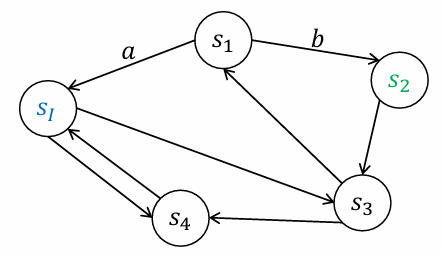
\includegraphics[width=0.5\linewidth]{Images/ricerca1.png}
\end{figure}

\subsubsection{La formulazione dei problemi}
La formulazione del problema è un \textbf{modello}, ovvero una descrizione matematica astratta.\\ Il processo di rimozione dei dettagli da una rappresentazione prende il nome di \textbf{astrazione} Per una buona formulazione del problema serve il giusto livello di dettaglio.
\\
Come faccio a specificare un problema di search?
\begin{itemize}
    \item \textbf{\textcolor{red}{Approccio esaustivo/esplicito} }: fornire il grafo degli stati in modo completo specificando tutte le transizioni possibili. Il più delle volte questa non è un'opzione percorribile a casua della natura combinatoria dello spazio degli stati.
    \item \textbf{\textcolor{blue}{Approccio implicito}}: possiamo specificare lo stato iniziale e la funzione di transizione in una forma \textbf{compatta}. Il grafo degli stati si "svela" man mano che le azioni vengono valutate.
\end{itemize}
Ci serve una procedura efficiente per ocntrollare se uno stato generato è il goal: \textbf{goal check}.

\subsection{Algoritmi di ricerca}
Un \textbf{algoritmo di ricerca} riceve in input un problema di ricerca e restituisce una soluzione o un'indicazione di fallimento. Considretiamo algoritmi ch esovrappongono un \textbf{albero di ricerca} al grafo dello spazio degli stati, formando vari cammini a partire dallo stato iniziale e carcando di trovarne uno che raggiunga uno stato obiettivo. Ciascun \textbf{nodo} nell'albero di ricerca corrisponde a uno stato nello spazio degli stati e i rami del'albero di ricerca corrispondo ad azioni. La radice dell'alvvero corrisponde allo stato iniziale del problema.
\\ È importante comprendere la distinzione tra spazio degli stati e albero di ricerca. Lo spazio degli stati descrive l'insieme degli stati nel mondo e le azioni che consentono le transizioni da uno stato a un altro. L'albero di ricerca descrive i cammini tra questi stati per raggiungere l'obiettivo. Nell'albero di ricerca possono esserci più cammini per raggiungere qualsiasi stato, ma per ogni nodo dell'albero c'è un cammino univoco per tornare alla radice.

\subsubsection{Obiettivi della ricerca}
Un algoritmo di ricerca \textbf{esplora il grafo delgi stati fin quando non trova la soluzione desiderata}. Nella versione di \textbf{fattibilità} quando viene visitato un nodo di goal viene restituito il percorso che ha portato a quel nodo. Nella versione di \textbf{ottimizzazione} quando viene visitato un nodo di goal, se quasiasi altro possibile percorso per quel nodo ha un costo maggiore, viene restituito il percorso che ha portato a quel nodo. \\ Non basta visitare un nodo di goal, l'algoritmo deve riscostruire il percorso che ha seguito per arrivarci: deve tenere traccia della sua ricerca. Tale traccia può essere mappata su un sotto-grafo di G, detto \textbf{albero} di ricerca.

\subsubsection{Come si valuta un algoritmo di ricerca?}
Possiamo valutare un algoritmo di ricerca lungo diverse dimensioni:
\begin{itemize}
    \item Correttezza
    \item Completezza
    \item Complessità in termini di spazio
    \item Complessità in termini di tempo
\end{itemize}
\subsubsection{Correttezza}
Garanzia che se l'algoritmo restituisce una soluzione, questa è conforme alle caratteristiche specificate nella formulazione del problema. \\ L'algoritmo dice che c'è una soluzione. È vero? E la soluzione che l'algoritmo ha calcolato conduce veramente ad un goal?
\subsubsection{Completezza}
Garanzia che se una soluzione esiste allora l'algoritmo la trova \textbf{sempre}. \\ L'\textit{algoritmo termina sempre? E se dice che non ci sono soluzioni, è vero?} \\
La completezza di solito si dimostra facendo vedere che la ricerca nello spazio degli stati + in grado di visitare tutti gli stati possibili, ap atto di concedere un temrpo arbitrariamente lungo.
\\ \textbf{Se lo spazio degli stati è infinito?} Possiamo chiederci se la riceca è \textbf{sistematica}:
\begin{itemize}
    \item se la risposta è \textit{sì} l'algoritmo deve terminare;
    \item se la risposta è \textit{no}, va bene se non termina ma tutti gli stati raggiungibili devono essere visitati nel limite: man mano che il tempo va all'infinito, tutti gli stati vengono visitati.
\end{itemize}

\subsubsection{Complessità spaziale e temporale}
\textcolor{blue}{Complessità spaziale}: come cresce la quantità di memoria richiesta dall'algoritmo di ricerca in funzione della dimensione del problema (caso peggiore)?\\ \textcolor{red}{Complessità temporale}: come cresce il tempo richiesto (numero di operazioni) dell'algoritmo di ricerca in funzione della dimensione del problema (caso peggiore)?
\\ \textbf{Trend asintotico}:
\begin{itemize}
    \item La complessità viene descritta con una funzione $f(n)$.
    \item Ai fini dell'analisi risulta conveniente adottare quella che si chiama la notazione "O-grande".
    \item $n$ di solito codifica la dimensione di una istanza del problema.
\end{itemize}
\section{Search: UCS e A*}
\subsection{Uniform Cost Seatch (UCS)}
Nell'albero di ricerca, teniamo traccia del nostro accumlato sul percorso dal nodo iniziale a ogni noto $V$: $g(V)$. Non consideriamo EQL. \\
L'UCS consiste nella selezione (espansione) del nodo con $g$ minore ancora da espolare (sulla frontiera). Goal check: se il \textbf{nodo selezionato per l'espandione} è un goal, mi fermo e restituisco la soluzione. \\
Ci si pone la domanda: abbiamo trovato il percorso ottimale per l'obiettivo? Per dare una risposta, possiamo ispezionare il grafico.
\begin{figure}[H]
    \centering
    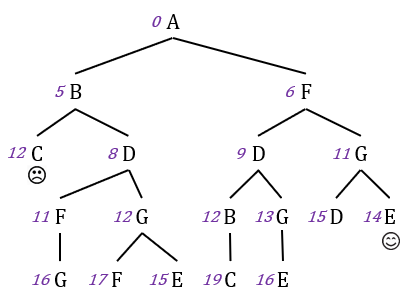
\includegraphics[width=0.5\linewidth]{Images/UCS.png}
\end{figure}
Come si nota dal grafico, sì, trova la soluzione ottimale.
\\
Anzi possiamo affermare che: \textcolor{red}{ogni volta che UCS \textbf{seleziona} per la prima volta un nodo per l'espansione, il percorso che, sull'albero di ricerca, porta a quel nodo ha un \textbf{costo minimo}}. 
\subsubsection{Ottimalità di UCS}
\begin{figure}[H]
    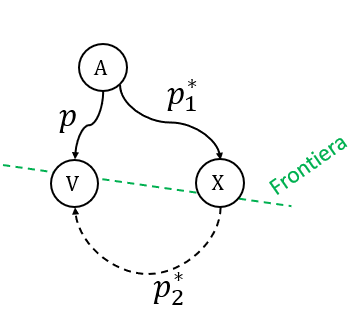
\includegraphics[width=0.5\linewidth]{Images/Ottimilita_UCS.png}
\end{figure}
\textbf{Overload della notazione}: estendo la notazione di $g$ rendendola applicabile anche ai path $g(X → Y → \dots → Z) = g(Z))$.
\\ \textbf{Ipotesi:}
\begin{enumerate}
    \item UCS seleziona per la prima volta dalla frontiera un nodo $V$ che è stato generato attraverso un percorso $p$;
    \item il percorso $p$ non è il percorso ottimo per raggiungere $V$: $p^* \neq p$;
\end{enumerate}
Dato il secondo punto e la \textcolor{green}{\textbf{separation property}} della frontiera, sappiamo che deve esistere un nodo $X$ sulla frontiera, generato attraverso un cammino $p_1^*+ p_2^*$. \\
$p*$ è il \textbf{path ottimo}, quindi $g(p_1^*)<g(p_1*)+\Delta{p_2^*} < g(p)$.
\\ I costi sono tutti positivi, quindi $g(p_1^*)<g(p_1*)+\Delta{p_2^*} < g(p) \Rightarrow g(p_1*) <g(p)$.
\\ Questo implica che $g(X)<g(V)$, \textcolor{red}{la prima ipotesi è violata}.
\\ Se quando selezioniamo per la prima volta un nodo scopriamo il percorso ottimo, non c'è motivo di selezionare lo stesso nodo una seconda volta, introduciamo quindi la lista dei \textbf{nodi espansi}: \textbf{EXL}.
\\ Ogni volta che selezioniamo un odo per l'estensione:
\begin{itemize}
    \item Se il nodo è già in EXL, lo \textbf{scartiamo}.
    \item Altrimenti lo estendiamo e lo insieriamo in EXL.
\end{itemize}

\begin{figure}[H]
    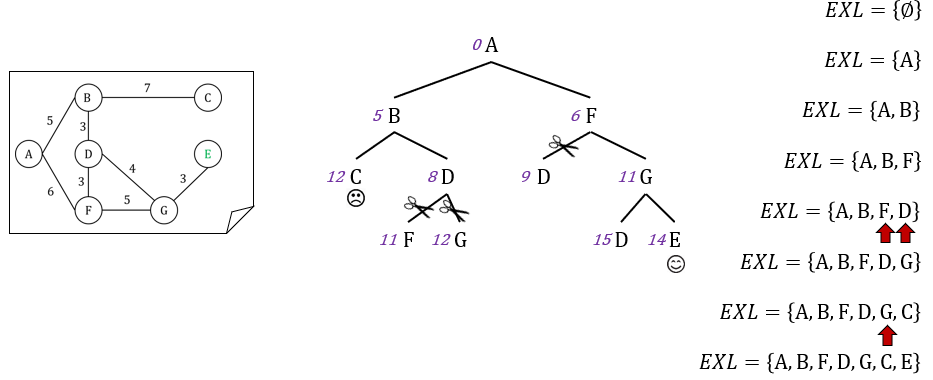
\includegraphics[width=1\linewidth]{Images/UCS_conEXL.png}
\end{figure}

\subsubsection{Implementazione}
\begin{figure}[H]
    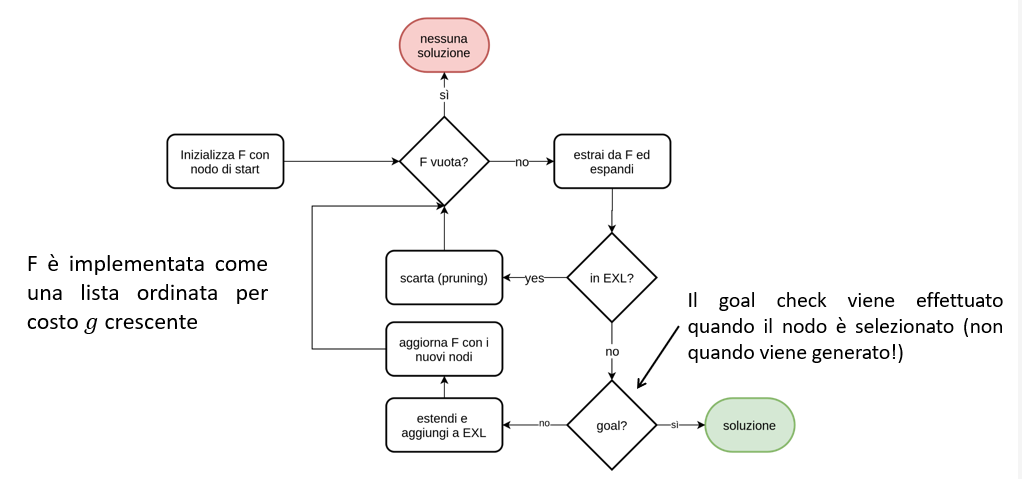
\includegraphics[width=1\linewidth]{Images/implementazione_UCS.png}
\end{figure}
\subsection{Ricerca informata}
\subsubsection{Ricerca non informata e non informata}
Gli algoritmi di ricerca decidono quale nodo espandere attraverso delle regole che applicano in funzione della conoscenza del problema e del processo di ricerca svolto fino al tempo presente.
\\ Una ricerca è \textcolor{blue}{\textbf{non informata}} se utilizza solo la conoscenza del problema che è specificata nella sua definizione.
\\ Una ricerca è \textcolor{red}{\textbf{informata}} va oltre alla definizione del problema sfruttando della conoscenza aggiuntiva: ciò che quel grafo, quelle connessioni e quei costi rappresentano nel mondo reale, oltre il formalismo agnostico che li esprime. 
\\ Dato un generico stato $S$, usando questa conoscenza, un algoritmo informato \textbf{stima} la bontà di $S$ attraverso una funzione $f(S)$ e guida la ricerca usando $f$.
\\Approccio \textbf{best-first}: espandere prima gli stati che hanno una $f$ migliore.
\\ Esistono diversi algorimti di ricerca best-first, la differenza la fa il \textbf{come $f$ è definita}.
\subsection{A*}
La forma più diffusa di ricerca best-first è la \textbf{ricerca A*}. La valutazione dei nodi viene eseguita combinando $g(n)$, il costo per raggiungere il nodo, e $h(n)$ (\textbf{euristica}), il costo per andare da lì all'obiettivo:
\[f(n)=g(n)+h(n)\]
Dal momento che $g(n)$ fornisce il costo di cammino dal nodo iniziale al nodo $n$, e $h(n)$ rappresenta il costo stimato del cammino più conveniente da $n$ all'obiettivo, risulta $f(n) = $ costo stimato della soluzione più conveniente che passa per $n$.
Se stiamo cercando di trovare la soluzione meno costosa, quindi una cosa ragionevole è provare per primo il nodo col valore più basso di $g(n)$ e $h(n)$. In effetti rilta che questa strategia è molto più che ragionevole, a patto che la funzione auristica $h(n)$
soddisfi certe condizioni, la ricerca A* è sia completa che ottima.
\subsubsection{Ammisibilità di A*}
A* è ottima se $h(n)$ è una \textbf{euristica ammissibile}, ovvero se $h(n)$ \textit{non sopravvaluta} mai il costo reale di una soluzione che passa per il nodo $n$.

\subsubsection{A* con EXL}
\begin{figure}[H]
    \centering
    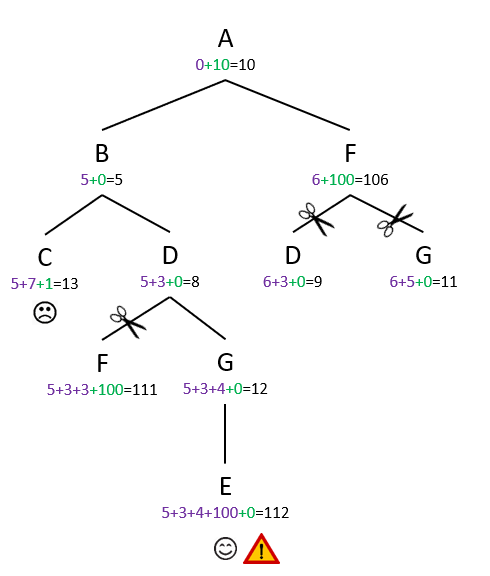
\includegraphics[width=0.4\linewidth]{Images/A_conEXL.png}
\end{figure}
Grazie all'ammisibilità manteniamo la stessa proprietà di ottimalità che abbiamo dimostrato con UCS: se non sovrastimiamo non possiamo scartare il path ottimo. \\
Se lavoriamo con EXL l'ammissibilità \textbf{non garantisce} l'ottimalità. Per risolvere ciò bisogna aggiungere all'euristica una proprietà più stringente: la \textcolor{red}{\textbf{consistenza}}.
\\ Siano $V$ e $U$ due stati connessi da una azione $a$. Una euristica $h$ è \textbf{consistente} se per ogni possibile coppia di $V$ e $U$ vale la seguente diseguaglianza: $h(V) \leq c(V, a, U)+h(U)$. (diseguaglianza triangolare)
\\
\begin{frame}{Disuguaglianza triangolare}
\end{frame}
Afferma che ogni lato del triangolo non può mai essere più lungo della somma degli altri due. 
\begin{figure}[H]
    \centering
    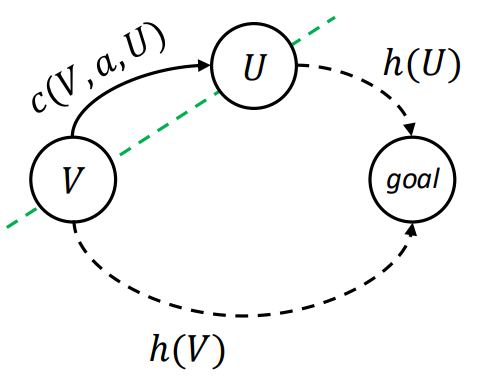
\includegraphics[width=0.25\linewidth]{Images/consistenza.png}
\end{figure}
\subsubsection{Ottimalità di A*}
Se assumiamo che $h$ sia consistente, possiamo costruire una dimostrazione per l'ottimalità di A*. \\ Cominciamo con il derivare una proprietà di $f$:
\begin{enumerate}
    \item Consideriamo due stati $V$ e $U$ connessi da un'azione $a$ che l'algoritmo ha generato uno dopo l'altro sull'albero di ricerca.
    \item Per definizione $f(U)=g(U)+h(U)$.
    \item Per definizione di $g$ e nostra azzunzione in 1, $g(U)=g(V) + c(V,a,U)$.
    \item Sostituiendo in 2: f(U)=g(V) + \textcolor{blue}{c(V,a,U)+h(U)}.
    \item Per la proprietà di \textcolor{blue}{\textbf{consistenza}} $c(V,a,U)+h(U) \geq h(V)$.
    \item \textcolor{green}{Sommando} $g(V)$ a entrambi i termini: \textcolor{green}{$g(V)+$} $c(V,a,U)+h(U) \geq \textcolor{green}{g(V)}+ h(V)$.
    \item \textcolor{red}{\textbf{$f(U) \geq f(V) \Rightarrow$}} \textbf{lungo ogni perorso nell'albero di ricerca la $f$ è monotono non decrescente}.
    \begin{figure}[H]
        \centering
        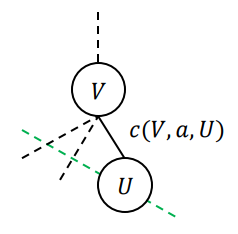
\includegraphics[width=0.25\linewidth]{Images/assimilitaA.png}
    \end{figure}
\end{enumerate}

Estendo la notazione di $f$ esplicitando il path su cui si calcola il costo $g$: $f(p,n)=g(p)+h(n)$
\\ \textbf{Ipotesi:}
\begin{enumerate}
    \item A* seleziona per la prima vola dalla frontiera un nodo $V$ che è stato generato attraverso un percorso $p$.
    \item il percorso $p$ non è il percorso ottimo per raggiungere $V$: $p^*\neq p$
\end{enumerate}
Dato 2 e la \textcolor{green}{\textbf{separation property}} della frontiera, sappiamo che deve esistere un nodo $X$ sulla frontiera che si trova sul cammino ottimo $p^*=p^*_1+p^*_2$ verso $V$;
\begin{figure}[H]
    \centering
    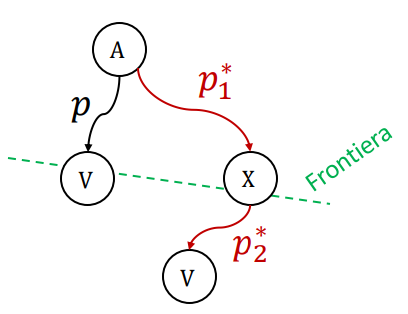
\includegraphics[width=0.50\linewidth]{Images/OttimalitaA2.png}
\end{figure}

\begin{enumerate}
    \item $g(p)>g(p^*)$ perch+ sia $p^*$ che $p$ sono path che portano a $V$, ma il primo è ottimo mentre il secondo no;
    \item $\textcolor{purple}{f(p^*, V)} \geq \textcolor{Turquoise}{f(p^*_1,X)}$ dalla consistenza di $h$ ($f$ monotona non decrescente);
    \item $\textcolor{red}{g(p)+h(V)} > \textcolor{purple}{g(p^*,V) + h(V)}$ sommando lo stesso termine ai membri di 1;
    \item $\textcolor{red}{f(p,V)}> \textcolor{purple}{f(p^x,V)} \geq \textcolor{Turquoise}{f(p^x_1,X)}$ mettedno insieme 3, 2 e la definizione di $f$;
    \item $f(p,V) > f(p^*_1,X)$ quindi $V$ non può essere stato scelto prima di $X$, \textcolor{red}{l'ipotesi 1 è violata}
\end{enumerate}
\subsection{Progettare un'eutistica}
Per capire come trovare un metodo per costruire buone euristiche, cerchiamo prima di capire come si può valutare una euristia: ci sono euristiche che sono migliori di altre? E come si stabilisce?
\\ Possiamo immaginare la nostra $h$ come un punto in un intervallo limitato:
\begin{figure}[H]
    \centering
    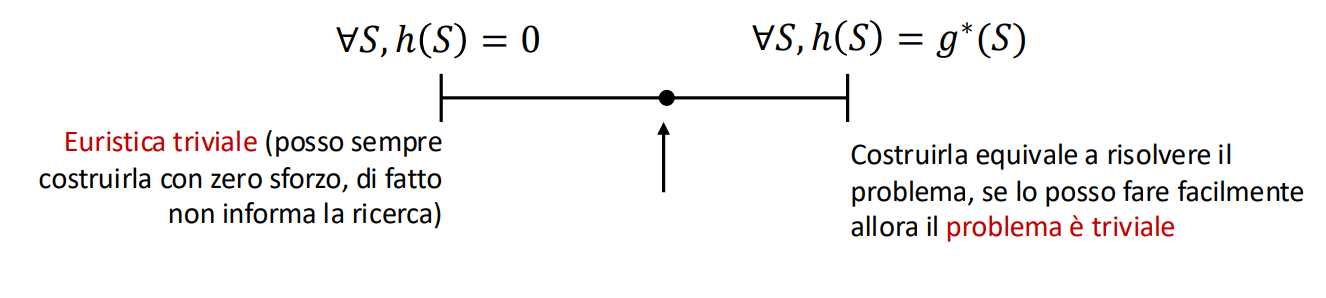
\includegraphics[width=1\linewidth]{Images/creareEuristica.png}
\end{figure}
Vorrei spingere il più possibile a destra il punto, mantendendo però l'\textbf{efficienza} nel computare $h$. Perchè?
\\ A* espande tutti gli stati $S$ tali per cui $f(S)<g^*(goal)$ cioè tutti gli stati $S$ tali per cui $h(S)<g^*(goal)-g(S)$. QUinsi se per ogni stato $S,h_1(S) \leq h_2(S)$ allora $h_2$ domina $h_1$ e A* con $h_2$ non espanderà ppiù nodi di A* con $h_1$ (sempre assumendo che entrambe le euristiche siano consistenti e calcolabili in tempo efficiente). \'E\ facile vedere che date due euristiche consistenti $h_1$ e $h_2$ dove nessuna domina l'altra, possiamo costruire una terza euristica che le domina entrambe: $h_3 = max\{h_1,h_2\}$
\\ Il principio "euristiche più grandi sono migliori" ci permette di valutare le euristiche o di combinarle, ma come si costruisce una euristica da zero?
\\ Tale compito sembra essere piuttosto complesso: l'euristica srutta la struttura di un problema e deve soddisfare una serie di vincoli. 
\subsection{Rilassamento di un problema}
Dato un problema $P$, un \textbf{rilassamento di P} è una versione più semplice di $P$ in cui alcuni vincoli sono stati rimossi.
\begin{figure} [H]
  \centering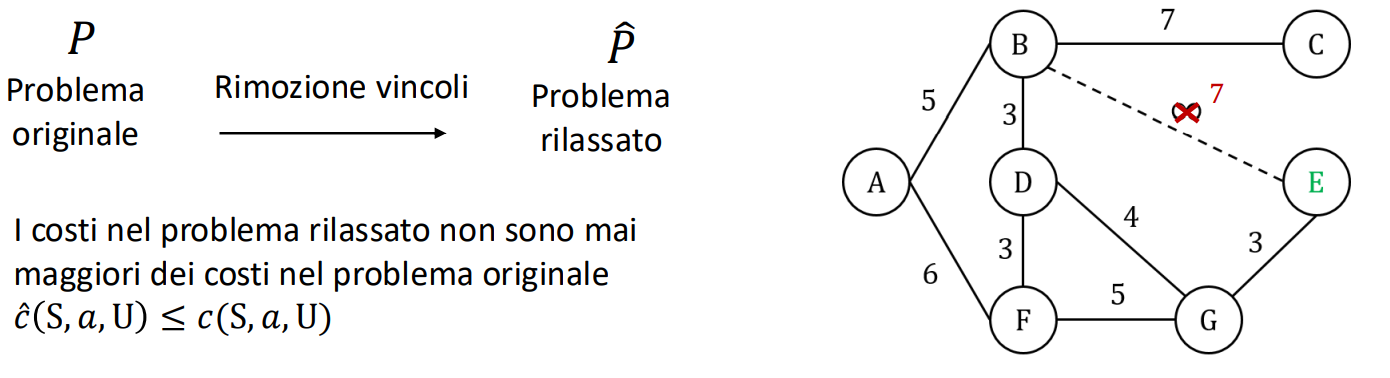
\includegraphics[width=0.75\linewidth]{Images/rilassamento.png}
\end{figure}
\textbf{Idea}:
\begin{enumerate}
    \item Costruire un rilassamento di $P$: $\hat{p}$.
    \item Eseguire A* (o un qualsiasi altro algoritmo di ricerca) sul problema rilassato e trovare il costo ottimo da ogni nodo $S$ per arrivare al goal: $\hat{h}^*(S)$.
    \item Assegnare $h(S) = \hat{h}^*(S)$ ed eseguire A* con tale euristica.
\end{enumerate}
Possiamo facilmente definire un problema di rilassamento, si tratta solo di rimuovere vincoli/riscrivere i costi. Ma cosa succede alle proprietà delle'euristica e all'ottimalità di A*?
\begin{enumerate}
    \item Nel problema rilassato risolvo per il costo ottimo da ogni stato $\hat{h}^*(S) \leq \hat{c}(S,a,U) + \hat{h}^*(U)$.
    \item Dalla nostra idea $h(S)\leq \hat{c}(S,a,U)+h(U)$.
    \item Dalla definizione di rilassamento $\hat{c}(S,a,U) \leq c(S,a,U)$.
    \item \textbf{L'euristica h è consistente} $h(S)\leq c(S,a,U)+h(U)$.
\end{enumerate}
\break
\section{Bounded Suboptimal Search e varianti di A* }
\subsection{Limiti di A*}
L'uso di euristiche ammissibili costituisce un vantaggio perchè garantisce l'ottimalità. Può essere anche essere un grosso limite per mancanza di flessibilità. 
\\ Consideriamo, ad esempio, una situazione in cui in frontiera non ci sono un gran numero di nodi:
\begin{itemize}
    \item ciascun nodo rappresenta un path verso il goal:
    \item ciascun path ha più o meno lo stesso costo, uno solo ha il costo minimo.
\end{itemize}
\begin{figure}[H]
    \centering
    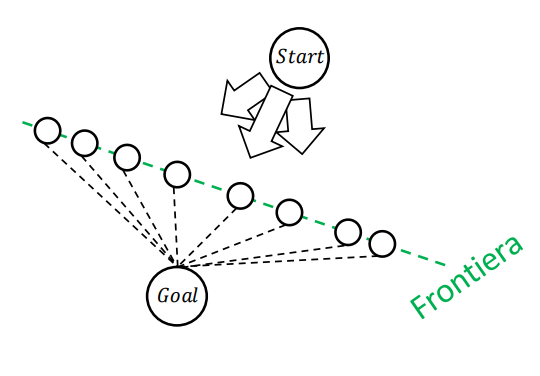
\includegraphics[width=0.5\linewidth]{Images/limitiA.png}
\end{figure}
\textcolor{red}{A* spenderà un sacco di tempo a distinguere il path ottimo tra tutti questi path che sostanzialmente sono equivalenti}. NOn si accontenta di un path sub-ottimale, anche quando il suo
costo dista di pochissimo dall'ottimo.
\\ \textcolor{blue}{Come possiamo equipaggiare A* con un po' di flessibilità?}.
\subsection{Focal Search}
Supponiamo di avere a disposizione una seconda euristica, \textbf{non ammissibile}, che chiamiamo $\hat{h}_F$.
\\ $\hat{h}_F(n)$ è una stima del \textbf{costo computazionale} necessario per completare la ricerca del percorso ottimo verso il goal.
\\ Ricordando che, in generale, in un problema di search le azioni \textbf{non} hanno costi uniformi, possiamo dire che dato un nodo $n$:
\begin{itemize}
    \item $h(n)$ stima ottimisticamente il costo rimanente da spendere per arrivare al goal;
    \item $\hat{h}_F(n)$ stima il numero di azioni ancora da compiere per arrivare al goal, ovvero la lunghezza della parte di soluzione ancora da costruire.
\end{itemize} 
Più è lunga la parte di soluzione da costruire, più lavoro dovrò fare per costruirla! Questa valutazione non è legata al costo rimanente.
\\ \textcolor{green}{\textbf{Esempio: Traveling Salesman Problem}}
\begin{figure}[H]
    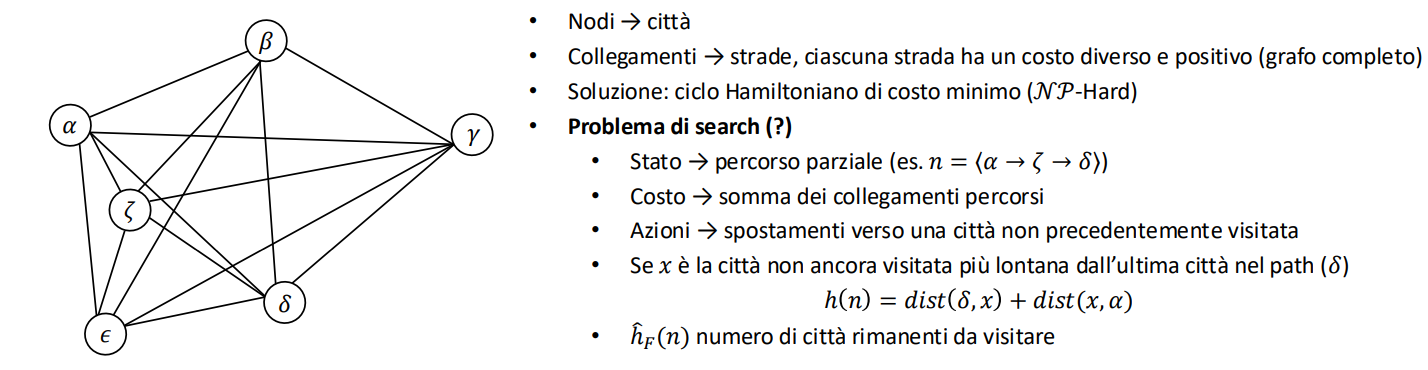
\includegraphics[width=1\linewidth]{Images/salesman.png}
\end{figure}
\begin{itemize}
    \item $F$: la lista di nodi in frontiera, quella usata da A*.
    \item $n_{best} = arg min_{n \in F} f(n)$
    \item $\omega \geq 1$, un parametro che scegliamo noi 
    \item $FOCAL \subseteq F$ sotto-lista definita cosi: \[FOCAL = \{n \in F | f(n) \leq \omega f(n_{best})\} \]
\end{itemize}
\begin{figure}[H]
    \centering
    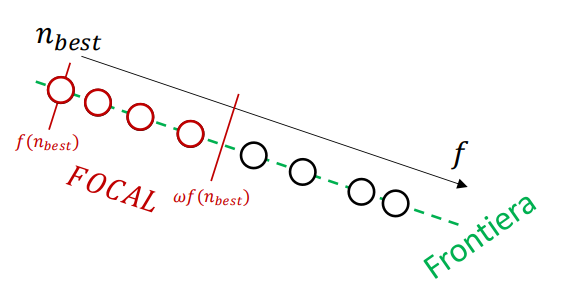
\includegraphics[width=0.5\linewidth]{Images/focal.png}
\end{figure}
\textbf{Regola di espansione}: scegliere la $FOCAL$ il nodo che minimizza $\hat{h}_F, n_{next} = arg min_{n \in FOCAL} \hat{h}_F(n)$.
\\ Tutto il resto resta uguale ad A*.
\\ \textcolor{red}{\textbf{Perdiamo l'ottimalità!}} Quando l'algoritmo seleziona per l'espansione un nodo di goal $e$ potrebbe non aver trovato il percorso ottimo
(potremmo non aver scelto il nodo con $f$ minima in frontiera e quindi potremmo aver saltato una linea di costo!)
\\ \textcolor{ForestGreen}{\textbf{La persita di ottimalità non è arbitrariamente grande}}, ma controllabile con il parametro $\omega$.
\subsubsection{Focal Search è una BSS}
\begin{itemize}
\item $e$: il nodo di goal selezionato da FOCAL (fa terminare la ricerca)
\item $n*$: il nodo che conduceva al goal su path ottimo, è in frontiera ma (assumiamo) non sia stato scelto
\item $OPT$ è il costo della soluzione ottima
\item $f(n^*)\leq OPT$ perchè $f$ usa un'euristica ammissibile
\item $f(n_{best}) \leq f(n^*)$ per definizione di $n_{best}$
\item $f(e)\leq \omega f(n_{best})$ per costruzione dell'algoritmo Focal Search
\item Mettendo insieme le disuguaglianze di cui sopra otteniamo: \[ g(e)=f(e)\leq \omega f(n_{best})\leq\omega f(n^*) \leq \omega OPT \Rightarrow g(e) \leq \omega OPT \]
\end{itemize}
Il costo della soluzione trovata da Focal Search può essere al più $\omega$ volte peggiore dell'ottimo
\\ BSS: Bounded Subotimal Search
\subsection{Problema del trashing}
La funzione $f$ può solo crescere. Questo implica, in $FOCAL$ search due effetti:
\begin{itemize}
    \item in $FRONTIER$ il nodo $n_{best}$ tenderà a stare a profondità bassa e quindi ad avere un valore alto di $\hat{h}_F$ (resta in FOCAL a lungo senza esser scelto)
    \item i nodi generati da una espansione tenderanno a non entrare in $FOCAL$ per molto tempo (fino a quando $n_{best}$ non viene rimosso).
\end{itemize}
Effetto "fisarmonica": $FOCAL$ viene svuotata, nel momento in cui viene rimosso $N_{best}$ viene riempita di nuovo, poi ancora svuotata, ... .
\\ Causa del problema: Focal Search usa $f$ per riempire $FOCAL$, questo sembrerebbe l'unico modo per garantire il bound della subottimalità, \textbf{ma non lo è}.
\\ Idea: usare $f$ solo per garantire il bound e usare, in ordine, $\hat{h}_F$, e una euristica "aggressiva" $\hat{h}$ per scegliere il nodo da espandere, EES (Explicit EStimation Search, 2011)
\subsection{Altri algoritmi di ricerca}
I vari concetti che definiscono gli algoritmi di ricerca visti in precedenza, possono essere visti come il loro building blocks.
\\ NUlla vieta di combinarli in modi alternativi per definire nuovi algoritmi di ricerca.
\begin{figure}[H]
    \centering
    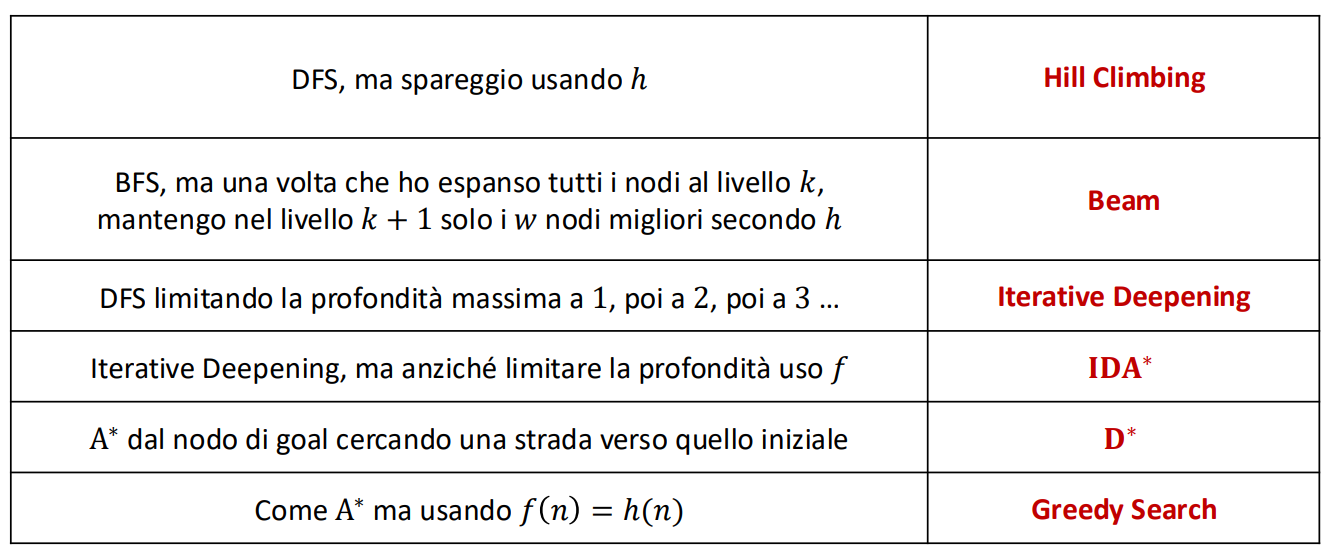
\includegraphics[width=1\linewidth]{Images/moreAlgoritmi.png}
\end{figure}
\section{Giochi: nozioni di base e Minimax}
\subsection{Adversarial Search}
L'adversarial search è una \textbf{ricerca con avversari} creata in un \textbf{ambiente competitivo} in cui vi sono due o più agenti con obiettivi in conglitto.
\\ Consiste in un ambiente multi-agente in cui gli obiettivi degli altri obiettivi non sono necessariamente concordanti con quelli del nostro agente di riferimento. In questi casi si parla di un sistema
multi-agente e l'interazione tra di esse può essere chiamata \textbf{gioco}.
\subsection{Giochi}
Un gioco è un problema di decisione \textbf{interattivo}. Ogni agente ha le proprie preferenze (utilità) individuali sugli stati del mondo. Le azioni di un agente influenzano l'ambiente e quindi, indirettamente, 
anche gli altri agenti. \\ Nel cercare una sequenza di azioni verso l ostato desiderato, l'agente da noi controlalto deve considerare le \textbf{strategie} degli altri decisori.
\\ Esistono diversi tipi di giochi:
\begin{itemize}
    \item 2 o \textit{n} giocatori;
    \item Agenti \textbf{razionali}, $\epsilon$-razionali;
    \item Struttura sequenziale: \textbf{turni}, azioni simultanee, ...;
    \item \textbf{Deterministico} o stocastico: tutte le azioni hanno effetti prevedibili?
    \item Stuttura dei payoff: \textbf{somma costante} o somma generica;
    \item \textbf{Informazione completa}/incompleta: i giocatori conoscono/non conoscono gli obiettivi e le azioni disponibili agli altri agenti;
    \item \textbf{Indormazione perfetta}/imperfetta: i giocatori sono/non sono informati di tutto quello che è succesos af ogni punto del gioco.
\end{itemize}
Lo studio del comportamente individuale dei singoli agenti si chiama \textcolor{red}{\textbf{teoria dei giochi competitivi}}.
\\Lo studio delle dinamiche nella formazione di coalizioni si chiama \textcolor{Aquamarine}{\textbf{teoria dei giochi cooperativa}}.
\\I giochi più studiati in IA sono quelli che gli studiosi di teoria dei giochi chiamano deterministici, a due giocatori, a turni, con \textbf{informazione perfetta} (completamente osservabile), \textbf{a somma zero} (ciò che a vantaggio di un giocatore danneggia l'altro).
\newpage
Consideriamo giochi formalizzati così:
\begin{itemize}
    \item \textbf{Stati}: $S=\{s_1,s_2,\dots\}$ insieme o \textbf{spazio} degli stati, dove $s_k \in S$ è lo stato \textbf{iniziali} (la situazione di partenza in cui trovano gli agenti e ambiente).
    \item \textbf{Giocatori e azioni possibili}: insieme di agenti $I=\{i_1,i_2\}$, insieme di azioni disponibili $A=\{a_1,a_2,a_3,\dots\}$.
    \item \textbf{Turni e azioni legali}: dato $s_k \in S$, $I(S_k)\in I$ è il giocatore che hanno diritto di compiere un'azione (turno) e $A(s_k)$ è l'insieme di azioni che può intraprendere.
    \item \textbf{Modello di transizione}: dato $s_k \in S$ e $a \in A(I(s_k))$, $f(s_k,a)\in S$ indica il prossimo stato del gioco e cioè il risultato della mossa $a$.
    \item \textbf{Stati terminiali}: dato uno stato $s_k$, $T(s_k)=1$ se $s_k$ è uno stato terminale, dove il gioco termina e un payoff viene inviato ad ogni giocatore; vale 0 altrimenti.
    \item \textbf{utilità}: dato uno stato terminare $s_t$, $u_i(s_t)$ è il payoff che il giocatore $i$ riceve in quello stato.
\end{itemize} 
Tutti questi punti prendono il nome di \textbf{meccanismo}.
\\ Questa formalizzazione implica: 2 giocatori, struttura sequenziale a turni alternati e azioni deterministiche.
\\ I giochi hanno anche altre caratteristiche:
\begin{itemize}
    \item \textbf{Informazione completa}: entrambi i giocatori hanno acceso al meccanismo, conoscono azioni possibili e utilità del proprio avversario.
    \item \textbf{Informazione perfetta}: dato uno stato corrente del gioco $s_j$ ogni giocatore ha accesso allo stato e alla sequenza di azioni che, a partire dallo stato iniziale, ha portato dino ad $s_k$.
    \item \textbf{A "somma zero"}: significa che in ogni stato terminale $s_t$ vale $u_1(s_t)+U_2(s_t)=0$.
    \begin{itemize}
        \item schema di competizione pura: il guadagno di un agente corrisponde ad una egual perdita dell'avversario;
        \item da un punto di vista matematico \textbf{è equivalente ad un gioco a somma costante} $u_1(s_t)+u_2(s_t)=C$
        \item Interpretazione: ogni giocatore paga una quota di $\frac{C}{2}$ per entrare nel gioco, poi $C$ viene ridistribuito a seconda dell'esito;
        \item Il gioco a somma costante $C$ può essere sempre trasformto in un gioco a somma zero rinormalizzando i payoff con una trasformazione affine;
        \item In un gioco a somma zero l'utilità del secondo giocatore è implicita, si indica solo con $u_1$, come se ci fosse un trasferimetno di utilità da $i_1$ a $i_2$. \textcolor{ForestGreen}{Esempio: $u_1=5 \rightarrow i_2$ paga $5$ a $i_1$, $u_1=-5 \rightarrow i_1$ paga $5$ a $i_2$}.
        \item Entrambi \textbf{massimizzano la loro utilità}, ma per $i_2$ (quello di cui non esplicitiamo l'utilità) vale: $max\{u_2\} = max\{-u_1\}= -min\{u_1\}$, quindi possiamo dire che cercherà di minimizzare $u_1$ così da ricevere il miglior posto possibile $-u_1$.
    \end{itemize}
\end{itemize} 
Il meccanismo descrive le "regole" del gioco, ma rappresenta solo una parte della sua descrizione.
L'altra parte è data dalle \textbf{strategie}.
\\ La strategia di un giocatore $i$ specifica il comportamente di quel giocatore in ogni possibile stato del gioco, dato $s_k$, tale per cui $I(s_k)=i,\sigma_i(s_k)$ è la strategia di $i$ nello stato $s_k$. Se la strategia coincide con una singola azione, quella da giocare in quel caso si chiama \textbf{strategia pura} $\sigma_i:\{s_k | I(s_k)=i\} \rightarrow A(s_k)$. Se invece la strategia è una distribuzione di probabilità su più azioni, si chiama \textbf{strategia mista} $\sigma_i:\{s_k|I(s_k)=i\} \rightarrow \Pi(A(s_k))$ (dove $\Pi(Q)$ è lo spazio di distribuzioni di probabilità sugli elementi di $Q$).
\\Ci concentreremo prinicipalmente sulle \textbf{strategie pure}
\\ \textbf{\textcolor{red}{Strategia ottima}}: quella strategia tale per cui ogni strategia diversa non introduce miglioramenti contro un avversario \textbf{infallibile}. 
\\Per ricolvere un gioco bisogna calcolare la strategia ottima.

\subsubsection{Albero di gioco}
Il meccanismo dà origine all'\textbf{\textcolor{red}{albero di gioco}}. Esso è un \textbf{albero di ricerca} che si ottiene sviluppando tutte le possibili sequenze di mosse alternate, in cui ogni nodo è un \textbf{\textcolor{red}{nodo di decisione}}: uno dei due giocatori deve fare la sua mossa.
\\ Ogni branch rappresenta un gioco (partita). Dallo stato iniziale fino a quello terminale dove il gioco termina e i payoff sono distribuiti, ogni foglia è uno stato terminale su cui indichiamo il payoff del giocatore $i_1$ (quello del giocatore $i_1$ è uguale all'oppsoto).
\textcolor{ForestGreen}{Esempio: il gioco del tris, Giocatore $i_1$: X, giocaotre $i_2$:0. Il branching massimo è b=9 e profondità massima d=9. Gli stati sono: \begin{itemize}
    \item $\leq 3^9=19683$
    \item rimuovendo gli stati illegali ne restano 5478, al netto delle simmetriche sussistono di fatto 5478, al netto delle simmetrie sussistono di fatto 765 diverse situazioni strategiche in cui decide.
    \end{itemize}
NUmero di nodi dell'albero di gioco: $\leq 1+9+(9*8)+(9*8*7)+(9*8*7*6)+ \dots = 986410$ se non facciamo ottimizzazioni è una stima ragionevole.
\\ Numero di giochi (ovvero i branch dell'albero o i suoi nodi terminali):\begin{itemize}
    \item $9*8*7*6*5*4*3*2*=9!=362880$
    \item numero esatto $255168$, al netto delle simmetrie $26830$.
\end{itemize}}
\begin{figure}[H]
    \centering
    \includegraphics[width=0.5\linewidth]{Images/alberoGioco.png}
\end{figure}
\subsection{Minimax}
Nei problemi di search l'albero di ricerca rappresentava/supportava il processo di inferenza per trovare una strada o la strada ottima per il goal. L'albero di gioco ha una funzione analoga: rappresenta/supporta il ragionamento strategico.
\\ Per adesso assumiamo che trovaer la strategia ottima sia un problema di search che tiene conto dell'avverario: \textbf{aversarial search}. L'approccio di base con cui si risolve la classe di giochi che stiamo considerando è dato dall'algormitmo \textbf{\textcolor{red}{minimax}}, sostanzialmente una DFS sull'albero di gioco con un \textbf{ritorno all'indietro} dei valori di utilità.
\\ È un approccio esautistivo e inefficiente che possiamo adottare solo per giochi di dimentisioni limitate, ma è un approccio esatto, corretto e completa; sta alla base dei metodi più sofisticati.
\\Introduciamo della notazione per semplificare la descrizione dell'algoritmo:
\\$I=\{\textcolor{red}{MAX},\textcolor{blue}{MIN}\}$, il giocatore $i_1$ si chiama \textcolor{red}{MAX} e il suo obiettivo nel gioco è ottenere un valore di utilità il più alto possibile. Il giocatore $i_2$ si chiama \textcolor{blue}{MIN} e il suo obiettivo è far sì che l'utilità di \textcolor{red}{MAX} sia la più bassa possibile
(implicitamente massimizza la sua utilità che, sotto l'assunzione di somma zero ,equivale a minimizzare l'utilità dell'avversario).
\\ Per semplicità \textcolor{red}{MAX} avrà sempre utilità $\geq 0$ (e di conseguenza quelle di \textcolor{blue}{MIN} saranno sempre $<0$).
Consideriamo giochi piccoli per ragioni di spazio, ma le considerazioni si generalizzano su ogni gioco.
\begin{figure}[H]
    \centering
    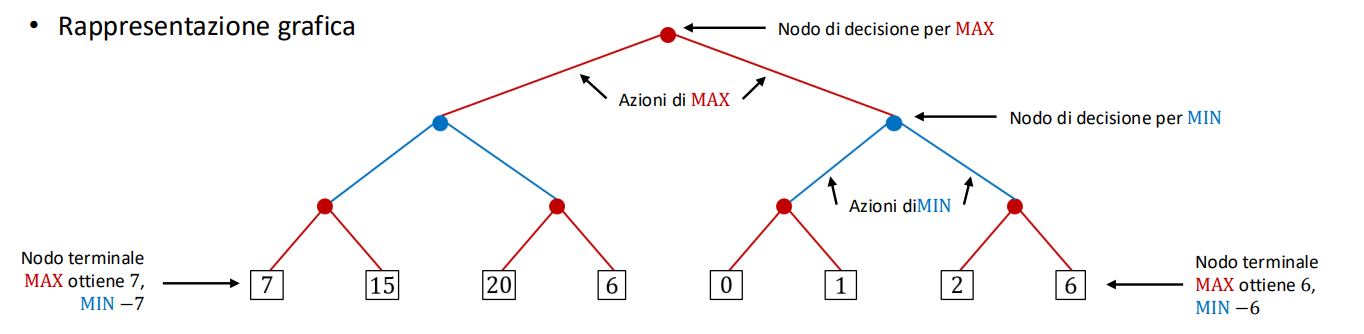
\includegraphics[width=0.75\linewidth]{Images/minmax.png}
\end{figure}
Procedimento:
\begin{enumerate}
    \item Eseguire una DFS sull'albero di gioco
    \item Riposrto all'indietro dei valori
\end{enumerate}
\begin{figure}[H]
    \centering
    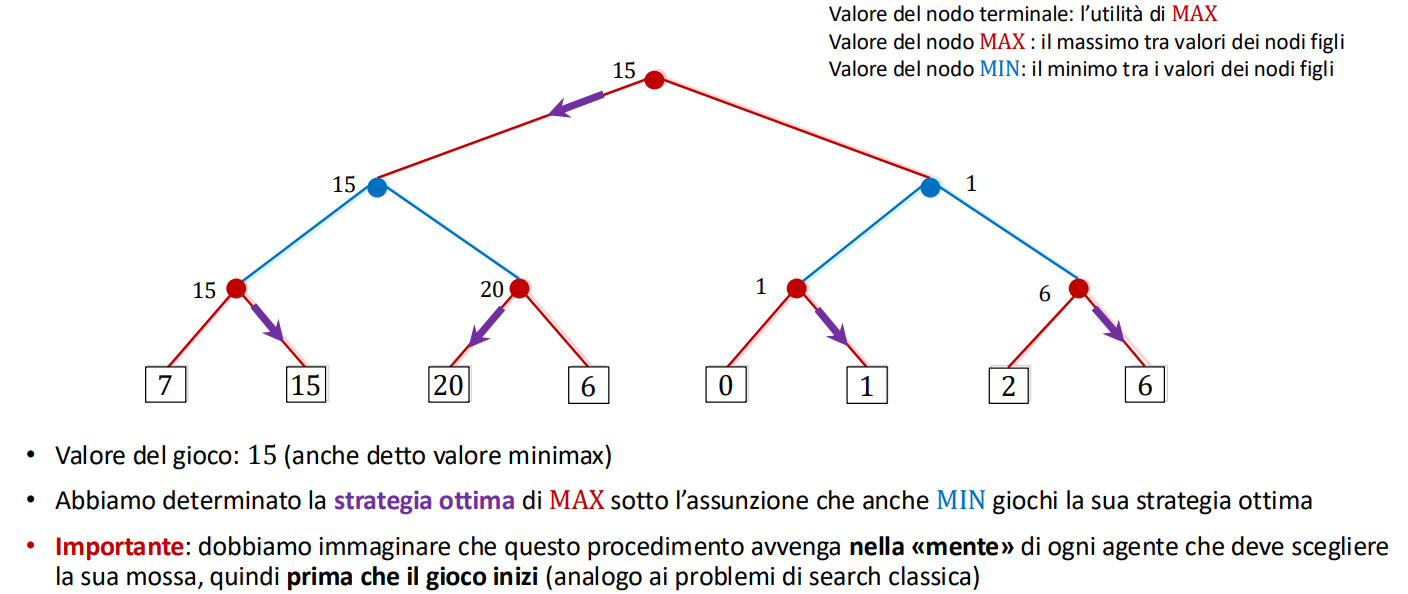
\includegraphics[width=0.75\linewidth]{Images/analisiMinMax.png}
\end{figure}
\end{document}
    